\documentclass[11pt]{article}
\usepackage[final]{acl}
\usepackage{times,latexsym}
\usepackage[T1]{fontenc}
\usepackage[utf8]{inputenc}
\usepackage{microtype,graphicx,amsmath,amssymb,booktabs,tabularx}
\graphicspath{{figures/}}
\hypersetup{pdftitle={Feature Survival and Intervention Preservation under Multilingual Weight Quantization},pdfauthor={Hemang Joshi, Eashaan Thakur, Shardul Joshi, Nikhita Ravi}}
\newcommand{\FP}{\mathrm{FP}}
\newcommand{\Q}{\mathrm{Q}}

\title{Feature Survival and Intervention Preservation\\under Multilingual Weight Quantization}
\author{Hemang Joshi \and Eashaan Thakur \and Shardul Joshi \and Nikhita Ravi\\
International Institute of Information Technology, Hyderabad}

\begin{document}
\maketitle

\begin{abstract}
Do the sparse autoencoder features used to interpret a language model remain useful after its weights are quantized? We study this question through paired activation measurements and controlled interventions in 27 languages, with three weight-quantization recipes on Gemma-2-2B, an original-RTN extension to Gemma-2-9B, and a limited Llama-3.2-1B check. Language-selective feature groups make consistent contributions to own-language next-token prediction: removing them causes excess loss beyond activity-matched controls in all 27 languages in both Gemma models. Their effects remain close to full precision at six bits and increase at four bits under RTN; GPTQ attenuates this increase and improves intervention fidelity. Activation and functional preservation nevertheless differ: at legacy INT4, only 13.2\% of a 1,487-feature sample passes the activation-survival cutoff, while effect fingerprints retain 99.7\% own-feature identity retrieval. Continuous activation correlation supplies modest positive predictive information, reducing language-held-out effect-similarity error by 3.1--4.4\% across six quantizer--precision conditions. A gain/noise decomposition clarifies its scale dependence, and crossed context--weight experiments locate intervention-transfer changes relative to numerical and direction controls. A held-out comprehension null bounds task relevance. The results support a controlled empirical account of feature and intervention preservation, with explicit distinctions between activation agreement, causal contribution and portability.
\end{abstract}

\section{Introduction}
Weight quantization changes the numerical representation of a language model without explicitly preserving the internal directions used to interpret it. Behavioral quality and internal preservation are therefore related but distinct evaluation targets. This matters especially in multilingual settings, where compression effects can differ by language and task \citep{marchisio-etal-2024-quantization}. A model can continue to perform a task while a particular feature changes, or preserve a recognizable feature effect while its activation correlation declines. An audit should measure these possibilities rather than define them to be the same.

Sparse autoencoders (SAEs) supply a practical basis for asking this question. They encode a residual state into sparse activations associated with learned decoder directions. Prior work identifies language-associated SAE features and manipulates them in full precision \citep{deng-etal-2025-unveiling}, while quantization studies compare the activations of a fixed SAE before and after weight rounding \citep{duan2026}. The remaining empirical issue is how those activation measurements relate to the effects of interventions, across languages and quantizers.

We evaluate several forms of preservation in a common experimental setting. The main study uses Gemma-2-2B with a frozen layer-12 Gemma Scope dictionary \citep{lieberum-etal-2024-gemma}, 27 FLORES-200 languages, and three simulated weight-only quantizers: the original RTN implementation, a matched RTN baseline and GPTQ \citep{frantar2023gptq}. We combine feature discovery, language-association retention, ablation and scaling, activation patches, individual effect fingerprints, and a crossed context--weight intervention design. An independently selected Wikipedia text panel checks transfer on fresh documents. A Gemma-2-9B original-RTN study supplies a larger-model extension; a Llama-3.2-1B check supplies evidence of heterogeneity in another model/dictionary setting.

Four final research questions organize this completed investigation:
\begin{description}
\item[RQ1:] How do language selectivity and resource tier relate to activation preservation under different quantizers?
\item[RQ2:] What do language-selective group interventions change across tasks and precision states?
\item[RQ3:] How informative are activation survival and language-association retention about intervention-effect preservation?
\item[RQ4:] How do context, downstream weights and generic sensitivity affect intervention portability?
\end{description}
These are retrospective synthesis questions. They organize the evidence without replacing the original hypotheses, analysis freezes or recorded decisions.

Our contribution is threefold. First, we provide controlled multilingual evidence that language-selective feature groups remain relevant to next-token prediction after compression, with quantizer-dependent effect changes and task-dependent behavioral relevance. Second, we characterize the relationship between activation and effect preservation: changed features often remain functionally identifiable, and continuous survival carries a small positive predictive signal. Third, we provide a measurement decomposition and a controlled intervention-transfer evaluation that separate activation gain, perturbation scale, context, downstream weights and generic sensitivity. The contribution is an empirical evaluation of these distinctions, rather than a new quantizer or a claim to recover complete language circuits.

\section{Related Work and Interpretive Framework}
\paragraph{Multilingual compression and language features.}
\citet{marchisio-etal-2024-quantization} document the dependence of multilingual quantization outcomes on task and evaluation. \citet{deng-etal-2025-unveiling} identify and intervene on language-associated SAE features, motivating our functional comparisons. Gemma Scope provides open dictionaries over Gemma 2 \citep{lieberum-etal-2024-gemma}. \citet{duan2026} measure frozen-SAE activation survival under RTN quantization. We extend activation auditing to functional relevance, effect preservation and quantizer comparisons. The existence of language-associated features or of activation drift is prior work; our emphasis is on their relationship under controlled weight perturbations.

\paragraph{SAE features are operational coordinates.}
Current SAE research does not establish that learned latents form a unique, complete inventory of the model's computations. \citet{leask2025canonical} demonstrate incompleteness and non-atomicity, while explicitly retaining the practical usefulness of SAEs. \citet{chanin2026sparse} show that sparsity choices affect disentanglement. These findings qualify semantic claims about a latent; they do not make an intervention along a specified direction unmeasurable. We therefore define a feature operationally as a learned coordinate and report the effect of the exact edit. Holding the dictionary fixed makes comparisons paired and interpretable without assuming that its coordinates are canonical mechanisms.

\paragraph{Functional evaluation and portability.}
\citet{makelov2025principled} motivate task-grounded evaluation without requiring a dictionary to recover exact ground-truth features. SAEBench shows that proxy gains need not translate into practical gains \citep{karvonen2025saebench}. Our comparisons similarly keep activation agreement, language association, prediction loss and effect fingerprints separate. Work on input-dependent quantization errors uses activation patching to localize changes \citep{chang-etal-2025-inputs}. Our crossed design evaluates the transfer of a fixed SAE edit, and uses alternate directions and small weight perturbations to distinguish feature-specific changes from generic sensitivity. This is a related evaluation question, not an assertion that those prior methods are invalid.

\section{Experimental Setting}
\subsection{Models, text and feature discovery}
The primary model is Gemma-2-2B \citep{gemma2024}, with a 16,384-latent JumpReLU SAE \citep{rajamanoharan2024} at the post-block layer-12 residual stream. Model inference uses bfloat16; SAE calculations and edits use float32. A BOS token is prepended and excluded, together with padding, from statistics and edits. A reproduction audit found substantial sensitivity to omitting BOS, motivating this fixed input regime; the retired implementation's results are excluded.

The FLORES-200 panel \citep{nllb2022} contains 27 languages, nine in each of three descriptive resource tiers (Appendix~\ref{app:languages}). Features are selected on the development split. Equal-budget activation measurements use 27,036 content tokens per language on devtest; functional loss experiments use 300 aligned devtest sentences per language. Resource tier is a grouping variable, not an intervention on training data. Shared aligned content controls a major comparison axis, while tokenization, scripts and feature activity remain relevant measured differences.

Let $p_{\ell f}$ be the firing rate of feature $f$ in language $\ell$. Selectivity is
\begin{equation}
 S_f=\frac{\max_\ell p_{\ell f}}{\operatorname{mean}_\ell p_{\ell f}}.
\end{equation}
Discovery uses a shuffled-language cutoff (95th percentile, 50 permutations), at least 50 peak tokens, panel rate at least $10^{-5}$, and stable peak identity in at least 80 of 100 resamples. There are 8,086 selected features; 6,663 establish a unique supported peak on FP devtest. A language group's K64 features are its highest-activation selective coordinates from dev. Controls are drawn from supported nonselective features and matched on log firing rate and log mean activation. The frozen K64 loss evaluation and graded scaling use three control draws (the group manifest stores up to five). Matching is close but imperfect, with documented K64 activity mismatches for Thai, Yoruba and Lao. Our estimand is the difference between these specified edits, not exclusive localization of a language faculty.

\subsection{Quantizers and additional evaluations}
The original, or \emph{legacy}, RTN recipe uses a scale shared across attention heads for corresponding attention coordinates and a rounding grid different from the later matched baseline. Matched RTN uses one scale per output channel and the same grid as GPTQ, without calibration. GPTQ uses approximate second-order calibration to compensate rounding error \citep{frantar2023gptq}; its pool contains 8,192 Wikipedia tokens per language (221,184 total), disjoint from the evaluation sentences. This comparison distinguishes grid/granularity changes from the remaining calibrated-method difference; it does not isolate compensation from calibration data.

All arms retain floating-point storage and inference, so the intervention is weight rounding rather than an integer-kernel deployment. Activation quantization is outside the measured setting. Activation/loss comparisons span INT8--INT4; the added functional and transfer comparisons use INT6 and INT4. INT16 and INT12 are small weight-perturbation references. Re-rounding bfloat16 weights can change them: INT16 is not a repeat of exactly identical arithmetic.

The external intervention-transfer panel uses fresh Wikipedia documents in six languages. Its articles are distinct from the calibration pool, though GPTQ calibration shares the Wikipedia domain. Belebele \citep{bandarkar-etal-2024-belebele} supplies 385 held-out questions per language in 18 calibration-qualified languages. Its primary outcome is normalized correct-option log-probability loss, with passage-clustered uncertainty; accuracy is reported separately.

Gemma-2-9B uses a layer-20, 16k Gemma Scope SAE and the 27-language, 300-sentence graded-scaling recipe under original RTN. Its imported per-state raw files were hash-checked and the downstream analysis reproduced byte-identically. This verifies the reported analysis of those files, rather than repeating GPU inference. The Llama-3.2-1B check uses a layer-12 TopK SAE with 14,336 latents and $k=48$, a different tokenizer and training setup. It is an additional system check, not a controlled isolation of model architecture.

\subsection{Evidence status and uncertainty}
Most FLORES experiments are exploratory: later questions were informed by earlier observations, and several analyses reuse examined sentences or contexts. Choices committed before a later stage was scored are reported as frozen-stage choices, not retroactively as independent preregistration. The original held-out Belebele family is confirmatory. The final synthesis introduces no new model experiment or hypothesis test.

We retain the uncertainty scheme of each analysis. Loss and group-effect intervals use paired sentence-cluster bootstraps, with the language set and selected groups fixed. The reviewed 9B--2B comparisons instead resample languages, paired across models. Feature-effect prediction uses language-held-out evaluation and language-bootstrap intervals. Transfer prediction holds out feature identities, and its crossed bootstrap resamples features and source sentences. These intervals address different sources of variation; a narrow conditional sentence interval is not a model-population guarantee. Unless stated otherwise, intervals are 95\% percentile intervals. We report estimates alongside the project's practical thresholds, rather than interpret a threshold miss as evidence of zero effect.

\section{Measurements and Intervention Design}
\subsection{Activation, association and functional effects}
Activation preservation is $R_{1f}^b=\operatorname{corr}_t(a_f^\FP(t),a_f^b(t))$. The historical survival rule is $R_{1f}^b>0.9$. Association retention instead asks whether an FP-established feature keeps its supported peak language. A correlation threshold and a peak-label decision therefore target different properties and populations.

For a residual state $x$, SAE activations $a$ and decoder directions $d_f$, an edit is
\begin{equation}
 x'=x+\sum_{f\in G}(a'_f-a_f)d_f.\label{eq:edit}
\end{equation}
This retains the reconstruction error rather than replacing $x$ by an SAE reconstruction. Ablation sets $a'_f=0$; scaling sets $a'_f=\alpha a_f$; a donor patch uses the aligned FP activation. Identity and sham edits validate the intervention path.

Let $h_\ell^b(G)$ denote the NLL increase caused by editing group $G$ relative to the unedited model in the same precision state. Excess language-group harm is
\begin{equation}
 E_\ell^b=h_\ell^b(G_\ell)-\frac{1}{R}\sum_{j=1}^{R}h_\ell^b(C_{\ell j}).\label{eq:net}
\end{equation}
Positive $E$ means this group edit affects own-language prediction more than its matched controls. Retention is $E_\ell^b/E_\ell^\FP$ for languages with a reliably positive FP effect. We distinguish the mean and median of per-language ratios from the ratio of mean effects: small denominators can separate them substantially.

Individual-feature F5 experiments summarize the change in output logits caused by an ablation as an effect fingerprint. Its cosine to the same feature's FP fingerprint is $W_1$. The 1,487-feature stratified sample is compared with different-feature and matched-direction controls. An INT16-derived reference cosine of 0.9489 defines the historical near-reference fidelity criterion. This threshold measures closeness to a small-perturbation reference, not whether a feature has any functional identity. Self-retrieval among fingerprints provides a complementary identity measure.

\subsection{Gain, noise and threshold-relative perturbation}
For centered FP and quantized activations $a,b$, ordinary least-squares decomposition gives
\begin{equation}
 b=ga+e,\quad g=\frac{\operatorname{Cov}(a,b)}{\operatorname{Var}(a)},\quad\operatorname{Cov}(a,e)=0.
\end{equation}
For nondegenerate cells,
\begin{align}
 r^2&=\frac{g^2\sigma_a^2}{g^2\sigma_a^2+\sigma_e^2},\label{eq:r}\\
 \lambda&=\log\frac{\sigma_e^2}{g^2\sigma_a^2}
 =\log\sigma_e^2-2\log|g|-2\log\sigma_a.\label{eq:lambda}
\end{align}
The sign of $r$ follows $g$. The identity shows that correlation reflects residual perturbation relative to signal scale; it is invariant to a noiseless gain change. It does not make correlation an invalid agreement measure.

We additionally measure encoder pre-activation perturbation in a feature's threshold units,
\begin{equation}
 \nu_f=\frac{\sqrt{\operatorname{mean}_{t:a_f^\FP(t)>0}(z_f^b(t)-z_f^\FP(t))^2}}{\theta_f},\label{eq:nu}
\end{equation}
where $z_f$ precedes JumpReLU and $\theta_f$ is its threshold. Streamed sufficient statistics recover $g$, residual noise, firing flips and $\nu$ without storing full token-by-feature arrays. Silent and degenerate cells are counted and reported.

\subsection{Crossed context--weight transfer}
An intervention's effect can change because its upstream context changes, because downstream weights change, or because they interact. For a fixed FP-amplitude decoder edit, let $D[p,s]$ be its mean centered logit effect with prefix state $p$ and suffix state $s$, each FP or quantized (Q). Each cell subtracts its own unedited baseline. Define
\begin{align}
 C&=D[\Q,\FP]-D[\FP,\FP],\\
 W&=D[\FP,\Q]-D[\FP,\FP],\\
 I&=D[\Q,\Q]-D[\Q,\FP]\nonumber\\
  &\quad-D[\FP,\Q]+D[\FP,\FP].
\end{align}
Thus $D[\Q,\Q]-D[\FP,\FP]=C+W+I$ exactly. For groups we compute analogous crossed contrasts directly on scalar excess-NLL effects; those quantities are in nats/token rather than vector norms. Norms and medians need not add. A fifth cell uses the quantized model's native amplitude. This distinguishes portability of a fixed intervention from a model's response to its own feature removal.

We repeat edits along a matched swapped decoder direction and three norm-matched random orthogonal directions. A per-direction INT16 reference defines a numerical/rounding floor; eligible real-direction items have FP effect norms above five floors. The main feature-level study contains 404 features and up to 16 contexts each (6,464 pairs), with 2,203 eligible pairs of 235 features. The normalized error is
\begin{equation}
 T=\frac{\|D[\Q,\Q]-D[\FP,\FP]\|}{\|D[\FP,\FP]\|+\mathrm{floor}}.
\end{equation}
Feature identities are split into calibration and held-out halves. Generic sensitivity, measured using the other directions at the same context, predicts transfer error beyond activation and gradient baselines. Shared source sentences across those halves are accounted for in uncertainty but do not turn the split into document-held-out validation.

\section{Results}
\subsection{RQ1: Preservation depends on scale and quantizer}
In the original BOS-masked RTN analysis none of the three initial tests rejects after Holm correction. The selective-minus-control survival differences are $-0.28$ and $-1.44$ percentage points at INT7 and INT6 (adjusted $p=0.514,0.128$). This does not establish equivalence. A stricter post hoc selectivity threshold ($S>5$, with the survival cutoff unchanged) gives $-7.16$ points at INT6; matching activation magnitude in ten bins reverses that contrast to $+4.58$. These sensitivities do not identify selective circuit destruction.

The legacy INT6 survival percentages are 69.4/90.6/95.1 for low/mid/high tiers. Controlling for activation scale attenuates the initial tier association. The later measurement audit finds a tier pattern already in the INT16 small-weight-perturbation reference; the RTN threshold-relative gradient changes little between INT16 and INT6/INT4. GPTQ's tier pattern depends on scale adjustment. Thus the measured disparities are meaningful descriptions of these representations, while their explanation is more conditional than a language-damage mechanism.

The quantizer contrast is substantial. At INT4, GPTQ improves the mean per-language survival rate by 17.83 points $[16.29,19.38]$ over legacy RTN and lowers its NLL increase by 0.461 nats/token $[0.348,0.595]$, in both cases improving all 27 languages. Against matched RTN the differences are $+11.86$ points $[11.18,12.50]$ and $-0.255$ nats/token $[-0.327,-0.193]$. These are paired language-bootstrap contrasts. Matched RTN itself improves on legacy RTN, showing why the implementation baseline matters. The small initial selective-feature contrast changes its significance classification under matched RTN and disappears under GPTQ. The supported conclusion is quantizer- and activity-dependent preservation, not universal selective vulnerability or the absence of multilingual disparities.

\subsection{RQ2: Language-group relevance persists, with task dependence}
Removing the K64 language group causes excess own-language NLL in all 27 languages in Gemma-2-2B. At FP the mean effect is 0.704 nats/token $[0.684,0.723]$, with median 0.262; every language's conditional interval is above zero. Graded suppression supplies convergent evidence: median excess harm rises from 0.022 to 0.090, 0.169 and 0.262 as the multiplier falls from 0.354 to 0.177, 0.088 and zero, with the ordered pattern in all 27 languages.

These effects largely persist at moderate compression. Under legacy RTN, median retention is 1.03 $[1.02,1.04]$ at INT6 and 1.54 $[1.43,1.62]$ at INT4 (sentence-cluster intervals). INT4 mean retention is 2.14 but the ratio of mean effects is 1.33. GPTQ reduces INT4 median retention to 1.22 $[1.14,1.24]$. Greater ablation harm means greater dependence on that edit in the compressed model; it is not improved language ability or a localization of all compression damage.

The reviewed 9B results support the same broad RTN precision pattern (Table~\ref{tab:9b}). FP excess harm is positive in all 27 languages; INT4 retention exceeds one in 26. Paired language-bootstrap differences between the two model sizes include zero: the INT4 median difference is $+0.048$ $[-0.777,0.838]$. This is useful scale-extension evidence, without establishing a size trend. The original 9B prediction list contains one reversed dose-order inequality and one selectivity criterion that cannot fail by construction. We report the empirical dose ordering and three informative prediction results, rather than count five independent confirmations. Appendix~\ref{app:9b} records the distinction.

\begin{table}[t]
\centering\small
\begin{tabular}{lrr}
\toprule
9B original RTN & Estimate & 95\% interval\\
\midrule
FP median harm & 0.270 & [0.197, 0.608]\\
INT6 median ratio & 1.019 & [0.978, 1.045]\\
INT4 median ratio & 1.586 & [1.238, 2.264]\\
INT4 mean ratio & 2.479 & [1.781, 3.368]\\
INT4 ratio of means & 1.474 & [1.263, 1.937]\\
\bottomrule
\end{tabular}
\caption{Reviewed Gemma-2-9B group effects. FP harm is in nats/token; ratios compare excess ablation harm with FP. All intervals here resample languages. Different ratio aggregations answer different questions. No 9B GPTQ result is included.}
\label{tab:9b}
\end{table}

The Llama check provides a boundary: its FP median effect is positive, 0.048 $[0.018,0.173]$, but only 21 of 27 languages have positive effects, and its INT4 behavior does not satisfy the frozen Gemma-consistency rule. Multiple aspects of the model/dictionary setup change together, so this identifies heterogeneity rather than its cause.

The held-out comprehension result is also informative. On 18-language Belebele, FP excess correct-option loss is $-0.0001$ nats/item $[-0.0035,+0.0031]$. Unedited accuracy is approximately 42.6\%; accuracy and log-probability loss are separate outcomes. The required positive FP effect is not established, so the frozen retention statements conditional on it are undefined. Larger positive-control interventions reduce accuracy by 1.2--6.0 points, and sham edits leave it unchanged; the controls include random nonselective sets and other languages' selective features. The test is sensitive to larger interventions but cannot exclude small group effects. GPTQ also yields a small, unresolved group contrast at INT4 where baseline accuracy is above chance.

Finally, FP donor patches to the language K64 group recover 2.6\% $[2.4,2.8]$ of the legacy INT4 loss gap, compared with 39.3\% $[38.5,40.0]$ for the full residual. GPTQ yields 2.0\% $[1.6,2.3]$ versus 41.4\% $[40.2,42.4]$. Original Study G does not meet its repair criteria, but a frozen extension on 562 fresh sentences detects a small legacy-RTN benefit at multiplier 1.1: $-0.00135$ nats/token $[-0.0020,-0.0003]$ (97.5\% interval; 20 of 27 languages improve). The two primary scaling ratios use Holm correction; the INT4-versus-FP contrast also meets its rule. On the 300-sentence main-study sample, GPTQ does not reproduce the fine-gain trend; the 562-sentence extension was not repeated with GPTQ. These findings support a small recipe-dependent improvement, rather than substantial repair. Patch recovery is not an additive mediation share. Together, the experiments establish text-prediction relevance while showing that task effects and repair efficacy require their own evidence.

\subsection{RQ3: Survival is informative, but not a functional verdict}
Activation agreement, peak-language association and effect geometry separate as precision falls. Among FP-established language features, 70.8\% keep their peak language at legacy INT4, despite much lower pooled correlation survival. The populations differ, so their rates should not be interpreted as competing estimates of one quantity.

Within the same 1,487-feature F5 sample, legacy INT4 activation survival is 13.2\%, while median effect cosine is 0.839 $[0.829,0.848]$; 99.9\% exceed the different-feature control and 99.7\% retrieve their own FP identity. Only 0.3\% meet the near-reference effect criterion. Features therefore change measurably yet retain distinctive effects (Figure~\ref{fig:agreement}). Matched-direction controls show that substantial drift is shared by other perturbations, qualifying a feature-specific damage interpretation. GPTQ raises INT4 median effect cosine to 0.923 (matched RTN: 0.875; legacy: 0.839).

\begin{figure}[t]
\centering
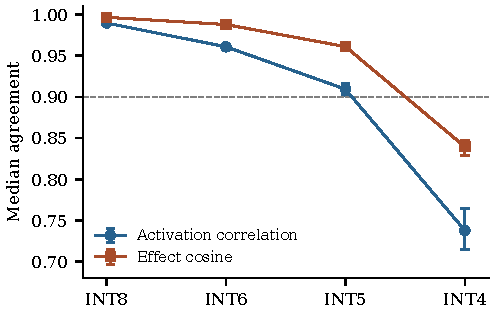
\includegraphics[width=\linewidth]{activation-effect.pdf}
\caption{Activation correlation and effect-fingerprint cosine on the same 1,487-feature legacy-RTN sample. Points are medians; bars are 95\% language-bootstrap intervals. The dashed line is the historical activation-survival cutoff, not a common decision rule for both metrics. Different trajectories motivate measuring both outcomes.}
\label{fig:agreement}
\end{figure}

We test incremental prediction on the 1,412 features whose INT16 fingerprints meet the reproducibility reference. Leave-one-language-out ridge models predict $W_1$ from activity, FP effect size, number of active sentences and edited positions; adding $R_1$ reduces held-out MAE by 3.1--4.4\%, with all six intervals above zero (Table~\ref{tab:prediction}). This is modest positive information, even though it falls below the project's 10\% practical convention. The Llama INT4 check similarly gives 4.2\% $[1.6,6.7]$; its INT6 estimate is unresolved. Binary association retention is less informative in the tested comparisons (descriptive legacy INT4 AUROC 0.506; GPTQ near-reference classification AUROC about 0.49 using the legacy labels). Continuous prediction and binary labels should not be conflated.

\begin{table*}[t]
\centering\small
\begin{tabular}{llrrr}
\toprule
Quantizer & Precision & Add activation correlation & Add gain and $\nu$ after correlation & Features\\
\midrule
Legacy RTN & INT6 & 4.4 [2.6, 6.2] & $-0.1$ [$-1.6$, 1.4] & 1,412\\
Legacy RTN & INT4 & 3.7 [2.3, 5.2] & 1.8 [$-0.3$, 3.7] & 1,412\\
Matched RTN & INT6 & 3.8 [1.6, 5.8] & $-0.4$ [$-1.6$, 0.9] & 1,412\\
Matched RTN & INT4 & 3.1 [1.8, 4.4] & 1.0 [$-0.5$, 2.5] & 1,412\\
GPTQ & INT6 & 4.1 [1.9, 6.2] & $-0.2$ [$-1.9$, 1.2] & 1,412\\
GPTQ & INT4 & 3.5 [2.1, 5.0] & 0.7 [$-1.5$, 2.8] & 1,412\\
\bottomrule
\end{tabular}
\caption{Relative reduction in held-out effect-similarity prediction MAE, in percent, with 95\% language-bootstrap intervals. The first column compares activity/effect-size baselines with those baselines plus activation correlation; the second adds gain and threshold-relative perturbation to that augmented model. Positive correlation gains are retained despite missing the project's 10\% convention. No additional gain/$\nu$ contrast separates from zero.}
\label{tab:prediction}
\end{table*}

The measurement sidecar supplies a more explicit interpretation. Over 214,506 FP-active language--feature cells, it reproduces prior correlations within $3\times10^{-8}$, retains identical survival counts, and verifies Equation~\ref{eq:r} to approximately $10^{-14}$ on nondegenerate cells. Median within-language rank correlations between $\lambda$ and log activation spread range from $-0.507$ to $-0.534$ across six conditions; for $\nu$ they range from $-0.004$ to $0.114$. The threshold normalization reduces dependence on spread, though not on peak activation (correlations 0.25--0.41). These are diagnostic properties, not proof of semantic invariance.

At INT4, median gain is 0.594/0.672/0.823 and the share of previously active tokens switched off is 50.0/42.9/27.0\% for legacy RTN/matched RTN/GPTQ. Those measurements show changes that correlation alone does not distinguish. Adding gain and $\nu$ beyond $R_1$ changes prediction MAE by $-0.4$ to $+1.8$\%, with every interval including zero. Their value here is interpretive decomposition, with no established extra prediction benefit. The combined answer is that activation survival carries information about effect preservation, while neither its cutoff nor a language-label decision supplies a complete functional verdict.

\subsection{RQ4: Portability changes through several pathways}
For the fixed FP-amplitude group edit at legacy INT4, median excess harm is 0.848 versus 0.263 at FP. The median absolute context term is 0.310 nats/token, compared with 0.104 for downstream weights and 0.071 for interaction. Using native quantized amplitudes instead reduces harm to 0.433. At INT6 the context and weight terms are small and similar, about 0.009 each. These are results for specified interventions in engineered states, not a unique natural decomposition of all quantization damage.

The single-feature logit endpoint differs: the weight-term norm exceeds the context-term norm. Legacy INT4 relative norms are 0.560 and 0.359, with interaction 0.315. This difference is coherent because the norm of a mean logit vector and a signed group-loss contrast measure different projections. We do not assign additive percentages to those norms.

Quantizer quality improves transfer in the same controlled sample (Table~\ref{tab:transfer}, Figure~\ref{fig:quantizers}). At INT4, effect cosine rises from 0.768 to 0.822 to 0.877 and normalized error falls from 0.664 to 0.572 to 0.476 across legacy RTN, matched RTN and GPTQ. These comparisons use identical eligible real-direction items. The displayed uncertainty is each arm's crossed-bootstrap interval; interval overlap is not itself a paired significance test.

\begin{table}[t]
\centering\small
\begin{tabular}{llrr}
\toprule
State & Quantizer & Cosine & Rel. error\\
\midrule
INT6 & Legacy RTN & 0.984 & 0.165\\
 & Matched RTN & 0.986 & 0.153\\
 & GPTQ & 0.990 & 0.132\\
INT4 & Legacy RTN & 0.768 & 0.664\\
 & Matched RTN & 0.822 & 0.572\\
 & GPTQ & 0.877 & 0.476\\
\bottomrule
\end{tabular}
\caption{Median fixed-intervention transfer on the same eligible real-direction items. The legacy INT16 small-weight-perturbation reference has cosine 0.998 and relative error 0.056. Table values summarize changed effects; they do not imply loss of feature identity.}
\label{tab:transfer}
\end{table}

\begin{figure}[t]
\centering
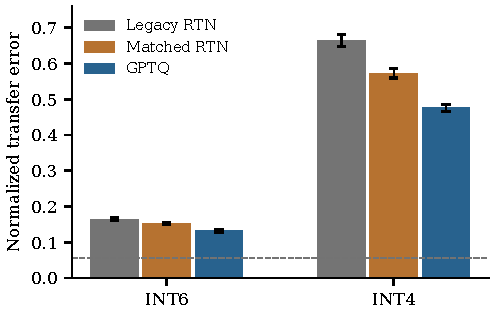
\includegraphics[width=\linewidth]{quantizer-transfer.pdf}
\caption{Median normalized transfer error by quantizer and precision on identical eligible items. Bars show 95\% crossed-bootstrap intervals for each arm. GPTQ preserves the tested intervention more closely, with remaining error above the INT16 reference.}
\label{fig:quantizers}
\end{figure}

Matched and random directions exhibit substantial common drift. Generic sensitivity measured with other directions predicts legacy INT4 transfer error beyond the strongest activation/gradient baseline, reducing held-out error by 21.5\% $[12.7,29.4]$. At INT6 the reduction is 10.9\% $[-1.2,21.4]$, so the original two-width utility criterion is not met. Similar predictive gains for the INT16 reference show that the predictor captures sensitivity to perturbations generally, not a quantization-exclusive mechanism.

The fresh Wikipedia panel repeats closer INT4 transfer under better quantization: median cosine is 0.754/0.808/0.876. Its prediction criterion is met at both widths for the RTN arms, whereas GPTQ meets it at INT4 and not INT6 (3\% $[-14,17]$ improvement at INT6, with error about 1.4 reference floors). This outcome is compatible with limited resolution when little transfer error remains; it is not evidence that GPTQ harms portability. Domain overlap with GPTQ calibration qualifies any attribution of the advantage.

Averaging over contexts raises apparent fingerprint agreement. In legacy INT4 the cosine of the averaged fingerprint exceeds the mean context-level cosine by 0.126 $[0.121,0.131]$, versus 0.0145 $[0.011,0.017]$ in the INT16 reference. Averaged and context-level portability are therefore different estimands. A useful audit states which one matters for the intended intervention.

\section{Discussion}
\paragraph{What the positive results establish.}
The controlled comparisons support a concrete account of preservation. The selected language groups affect own-language next-token prediction; that dependence is broadly retained at moderate compression, and its increase under strong RTN compression appears in both Gemma sizes. Better quantization improves survival and functional fidelity in the 2B matched setting. Many features remain identifiable by their effects despite substantial activation drift. Continuous survival has a modest predictive contribution, while decomposition and alternate-direction controls clarify which aspects of a change it measures. These conclusions rest on observed contrasts and do not require exhaustive model or dictionary coverage.

\paragraph{What the negative results contribute.}
The initial selective-vulnerability hypothesis is not established, the held-out comprehension intervention has no resolved FP effect, and the tested patches and gains offer limited repair. Those outcomes specify where an explanation or intervention does not earn its proposed interpretation. They coexist with strong group-loss effects and improved fidelity under GPTQ. The task null is a finding about this edit and endpoint; failure of a practical prediction threshold is a finding about its target, not evidence that the observed predictor contains no information.

\paragraph{A measurement contribution in current mechanistic interpretability.}
SAE nonuniqueness, mixed features and imperfect semantic grounding are active field-wide issues. Our answer is to keep the coordinate system fixed, define each intervention precisely and test it against controls and functional endpoints. This yields causal evidence about the specified edit without asserting that the latent is an atomic, exclusive circuit. Conversely, noncanonicity alone does not refute the effect of that edit. The results motivate joint reporting of activation agreement, effect fidelity, task relevance and numerical reference behavior when transferring interpretability findings to compressed models.

\section{Conclusion}
Multilingual feature preservation under quantization has several measurable components. In the tested settings, language-selective groups retain causal relevance for text prediction, quantizer choice materially affects their preservation, and activation drift can coexist with recognizable functional identity. Activation correlation provides a modest positive predictive signal, while gain/noise and context--weight decompositions expose changes that a survival label does not summarize. Reporting these outcomes together provides a more informative empirical account of intervention portability than treating either behavioral quality or feature survival as a sufficient certificate.

\section*{Limitations}
\paragraph{Scope and generalization.}
The most extensive experiment is Gemma-2-2B at one layer with one fixed SAE; Gemma-2-9B extends original-RTN group effects, and Llama supplies a narrower different-system check. This coverage bounds generalization to other model/dictionary combinations. It does not invalidate paired effects in the systems studied. We evaluate simulated weight quantization, not deployment kernels, activation quantization or all compression methods. The 9B GPTQ arm has not been run and supplies no evidence; matched-RTN 9B and a separate arithmetic-precision audit are possible extensions, not inputs to the current conclusions.

\paragraph{Representation and intervention validity.}
A frozen SAE is a measurement basis whose coordinates may mix or split concepts. We estimate effects of those coordinates rather than exclusive natural circuits. Activity matching and direction controls reduce alternative explanations but do not equalize every geometric property. Large edits can create atypical states, and fixed FP-amplitude edits differ from native ablations. The crossed design is useful precisely because that intervention choice is explicit. Patch recovery cannot be interpreted as an additive causal share of total model degradation.

\paragraph{Sampling, dependence and inference.}
Most studies reuse examined FLORES data, and F5 uses a stratified feature sample. Frozen later-stage choices improve transparency without supplying fresh-data confirmation. Language-held-out prediction is not document-held-out prediction; feature-held-out transfer contexts can share source sentences. Bootstrap intervals describe the specified clusters conditional on other fixed choices, not uncertainty across model training seeds. Twenty-seven languages and the six-language external panel give finite resolution for language-level adjustments; GPTQ tier conclusions remain adjustment-sensitive. Three-arm exploratory comparisons have no project-wide multiplicity guarantee. These limits qualify confidence and breadth, while leaving directly measured contrasts reportable.

\paragraph{Audit record and reproducibility.}
The 9B analysis reproduces the imported raw-file outputs but not GPU inference. Its prediction-definition defects are explicitly recorded in Appendix~\ref{app:9b}. Numerical gates, identity/sham checks and small-weight-perturbation references constrain implementation errors, but do not prove semantic completeness. Code, analysis freezes, result tables and provenance are retained in the project repository. Large raw outputs are stored in a private artifact dataset; independent access currently requires the authors to share it. Public artifact availability is not claimed.

\bibliography{references}

\clearpage
\appendix
\section{Language Panel}\label{app:languages}
The descriptive tiers contain nine languages each. High: English, German, Spanish, French, Portuguese, Russian, Chinese, Japanese and Korean. Mid: Hindi, Bengali, Tamil, Turkish, Vietnamese, Indonesian, Thai, Polish and Ukrainian. Low: Kannada, Telugu, Yoruba, Sundanese, Amharic, Igbo, Hausa, Khmer and Lao. These labels summarize the study's resource grouping; they are not a controlled intervention on model training exposure.

The 27 parallel languages provide aligned sentence content but different token counts per sentence. Equal-budget activation streams and aligned-sentence functional studies consequently have different token populations. All feature-survival percentages retain their original population definitions. F5's 1,487-feature stratified population, its 1,412 reliable-fingerprint subset and the transfer study's eligible feature--context pairs must not be pooled as independent estimates of one rate.

\section{9B Review and Prediction Definitions}\label{app:9b}
The original-RTN 9B files use the same Study G analysis as 2B. Review checked file hashes, state metadata, sentence identifiers and byte-identical regeneration of curves and reports. Three informative predictions are supported: positive FP excess harm, near-FP INT8/INT6 effects, and larger INT4 retention. The frozen dose-order inequality is written in the opposite direction to increasing suppression harm: its literal ordering holds in zero languages, while the physically intended harm ordering holds in all 27. We do not silently rewrite the frozen criterion. The final paper reports the observed monotonic dose response and this definition error together.

A second criterion asks for a selectivity statistic above 1.3 among features already selected above a larger cutoff. It therefore cannot serve as independent confirmation. The reviewed statement separates this circular criterion from the empirical group effects. The model-size comparison uses language-paired resamples and finds no resolved difference in effect magnitude, despite matching broad precision patterns. Those checks support the reported extension with a narrower interpretation than its imported headline verdict.

\section{Practical Conventions and Uncertainty}
The survival cutoff 0.9, near-reference effect cosine 0.9489, five-floor transfer eligibility, 10\% prediction improvement target and tier equivalence bounds are operational conventions chosen for this project. They facilitate reproducible decisions but do not define universal boundaries between preserved and destroyed features or between information and no information. Quantitative estimates and intervals remain the results when a threshold label changes.

For example, the reliable-population correlation predictor improves MAE by 3.1--4.4\%, with every interval above zero, yet fails the 10\% practical target. By contrast, adding gain and perturbation after correlation has intervals including zero in all six cells. These statements have different inferential meanings. Likewise, a feature can fail the near-reference cosine criterion while retrieving its own FP fingerprint among alternatives. A report of measurable drift should not erase that retained identity.

The new streamed audit covers 214,506 FP-active language--feature cells. Depending on condition, 4--239 cells are excluded from the gain/noise identity check because of degeneracy; silent and clipped cases remain counted in the population tables. Reproduction of earlier correlations and an algebraic identity validates the measured quantities and implementation consistency, rather than establishing that any one quantity fully measures semantic function.

\section{Reproduction and Evidence Map}
This manuscript introduces no new inference runs or hypothesis tests. Figures are rendered directly from committed CSV and JSON estimates with their existing intervals. The accompanying evidence map records each numerical block's source, population, uncertainty and status; the source register records the primary literature inspected for the interpretive framework. The original hypotheses, analysis freezes, generated verdicts and dated histories are retained separately from the final synthesis.

All main 2B quantizer analyses and the measurement sidecar are complete. The missing 9B GPTQ extension is reserved for a later addendum and is absent from all tables and claims here. Broader model, SAE and kernel evaluations would extend the study's external validity; the completed intervention and measurement results stand on their specified comparisons.
\end{document}
